Trong phần này, tác giả trình bày các kết quả đạt được từ hai giai đoạn chính: 
(i) thu thập và xử lý dữ liệu cảm biến từ các tư thế ngủ khác nhau; 
(ii) huấn luyện mô hình học máy và triển khai mô hình tối ưu lên vi điều khiển nhằm đánh giá tính khả thi của giải pháp trên thiết bị biên.

\section{Hệ thống thực nghiệm}

\begin{figure}[htbp]
    \centering
    \begin{subfigure}[b]{0.45\linewidth}
        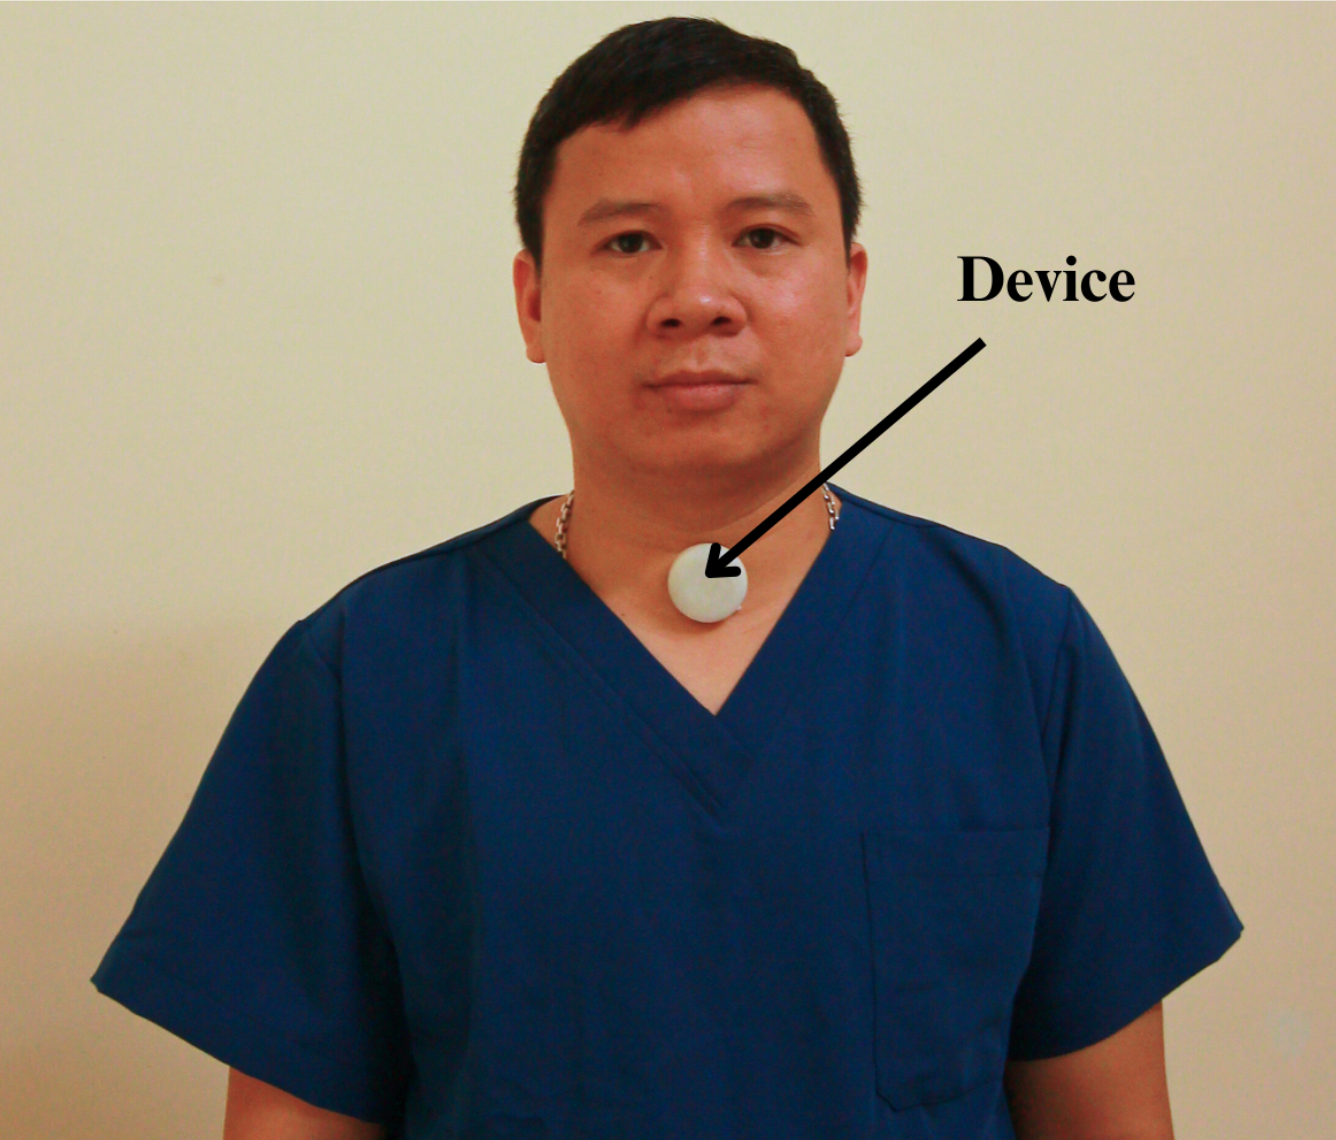
\includegraphics[width=\linewidth,height=6cm,keepaspectratio]{images/sleepdive2.png}
        \caption{}
        \label{fig:device_position}
    \end{subfigure}
    \hfill
    \begin{subfigure}[b]{0.45\linewidth}
        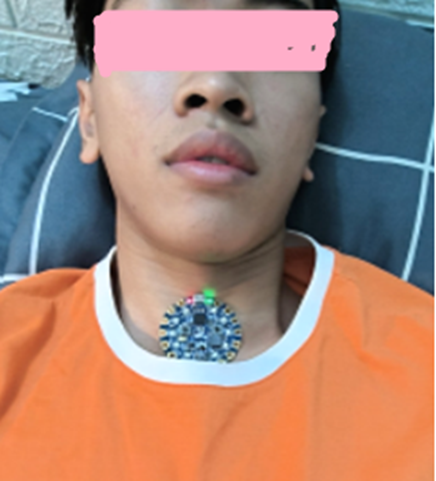
\includegraphics[width=\linewidth,height=6cm,keepaspectratio]{images/thucnghiem.png}
        \caption{}
        \label{fig:practical_test}
    \end{subfigure}
    \caption{Hệ thống thử nghiệm: (a) vị trí đặt thiết bị cảm biến; (b) minh hoạ thực nghiệm thực tế trong tư thế nằm.}
    \label{fig:experiment_system}
\end{figure}

Tác giả đã hoàn thiện việc lập trình firmware cho bộ vi mạch cảm biến 
tích hợp vi điều khiển NRF52840 và cảm biến gia tốc ba trục LIS3DH. 
Firmware được xây dựng sử dụng ngôn ngữ C/C++ trên nền tảng Arduino Core, 
tối ưu hóa để vận hành ổn định trong môi trường năng lượng thấp và 
hỗ trợ giao tiếp không dây chuẩn Bluetooth Low Energy (BLE).

Để đảm bảo khả năng hoạt động liên tục trong suốt một đêm ngủ 
(tối thiểu 8 giờ), hệ thống được thiết kế sử dụng pin cúc áo CR2032, 
với dòng tiêu thụ trung bình được đo đạt dưới 8 mA trong chế độ 
ghi nhận liên tục và truyền dữ liệu định kỳ.

Mã nguồn firmware bao gồm các khối chức năng chính: 
khởi tạo cảm biến, hiệu chỉnh dải đo và tần số lấy mẫu (10~Hz), 
lọc nhiễu đầu vào (bằng kỹ thuật trung bình trượt), 
đóng gói dữ liệu,
và truyền dữ liệu qua BLE đến ứng dụng Android. 
Ngoài ra, tác giả cũng tích hợp cơ chế báo hiệu bằng LED để xác nhận 
trạng thái hoạt động của thiết bị (kết nối, truyền dữ liệu, và lỗi).
Kết quả thử nghiệm thực tế cho thấy hệ thống hoạt động ổn định 
trong suốt thời gian ghi nhận dữ liệu qua đêm, không xảy ra hiện tượng 
rớt kết nối hay tràn bộ đệm dữ liệu. Toàn bộ dữ liệu thu được được đồng 
bộ theo thời gian thực tới ứng dụng di động, phục vụ cho các giai đoạn 
xử lý tín hiệu và huấn luyện mô hình học máy ở các chương sau.


Một trong các nhiệm vụ chính mà tác giả thực hiện là phát triển ứng dụng 
di động phục vụ cho quá trình thu thập, hiển thị và xử lý dữ liệu. 
Dựa trên phản hồi từ nhóm nghiên cứu, tư vấn khoa học của Thầy PGS.TS. Mai Anh Tuấn, tư vấn
y khoa của Thầy GS.TS. Dương Quý Sỹ,
ứng dụng được thiết kế với tiêu 
chí giao diện thân thiện, thao tác đơn giản và tính năng tập trung vào 
mục tiêu thử nghiệm.

Sau khi cài đặt, người dùng có thể đăng nhập hoặc đăng ký tài khoản 
thông qua giao diện như được thể hiện trong Hình~\ref{appAuth}. 
Với người dùng mới, quá trình đăng ký yêu cầu xác thực địa chỉ 
email nhằm đảm bảo bảo mật và hỗ trợ tính năng khôi phục tài khoản.
Hình ~\ref{app_cate} là giao diện khi người dùng đăng nhập thành công, 
bao gồm các tính năng: Kết nối BLE và đọc dữ liệu, chuyển người dùng, 
xem thông tin người dùng v.v.
Hình ~\ref{listble} thể hiện danh sách BLE có thể kết nối và 
dịch vụ kết nối với phần cứng đã được nhắc tới bên trên.


\begin{figure}[htbp]
    \centering
    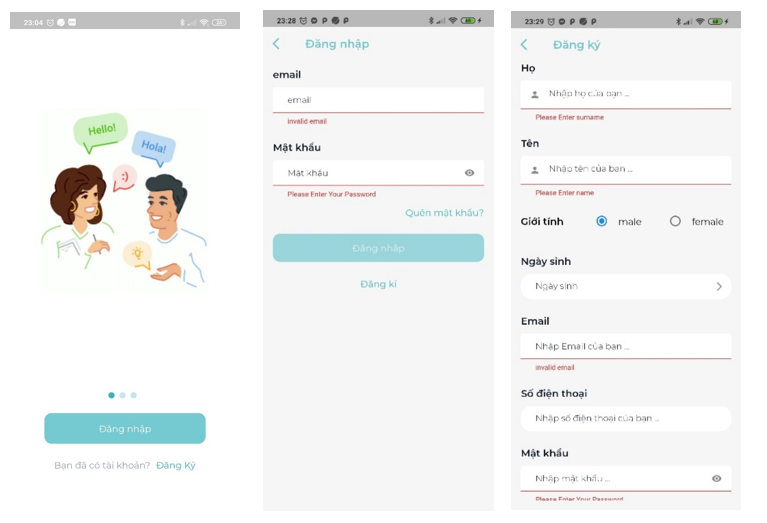
\includegraphics[width=0.8\linewidth]{images/appAuth.png}
    \caption{Giao diện chức năng đăng ký và đăng nhập}
    \label{appAuth}
\end{figure}

\begin{figure}[h!]
    \centering
    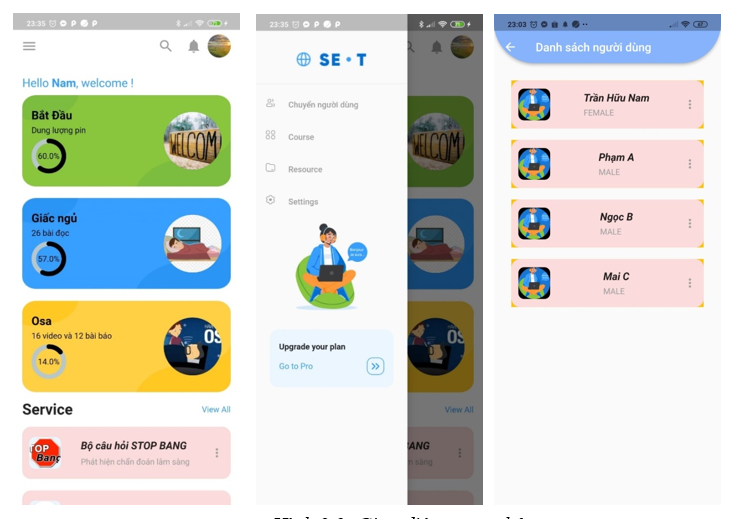
\includegraphics[width=0.8\linewidth]{images/app_cate.png}
    \caption{Giao diện trang chủ}
    \label{app_cate}
\end{figure}


\begin{figure}[htbp]
    \centering
    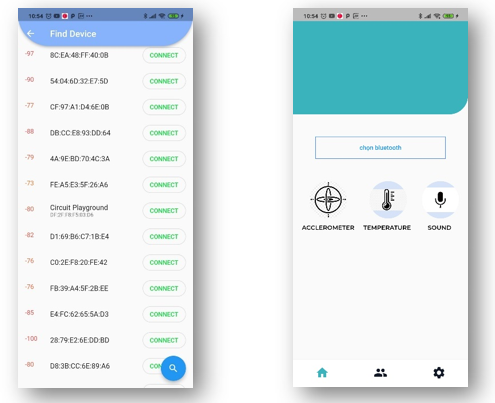
\includegraphics[width=0.5\linewidth]{images/app_ble.png}
    \caption{Giao diện màn hình danh sách BLE và chi tiết các dịch vụ kết nối với phần cứng}
    \label{listble}
\end{figure}

Hình~\ref{appsleep} minh họa giao diện của các chức năng hỗ trợ người 
dùng trong quá trình sàng lọc nguy cơ ngưng thở khi ngủ và cung cấp 
thông tin về chất lượng giấc ngủ. Giao diện đầu tiên (từ trái sang) 
hiển thị mục "Hỏi – Đáp về Giấc Ngủ", nơi người dùng có thể tra cứu 
các thông tin được tổng hợp từ chuyên gia trong lĩnh vực y học giấc ngủ. 
Giao diện thứ hai trình bày tập hợp các công cụ đo lường phổ biến như 
thang điểm Epworth, STOP-BANG, chỉ số khó có thể duy trì sự tỉnh táo 
(ESS), và các bộ câu hỏi dành riêng cho trẻ em hoặc đánh giá chất lượng 
giấc ngủ theo thang điểm Pittsburgh (PSQI).
Giao diện thứ ba mô tả chi tiết một bộ câu hỏi sàng lọc nguy cơ ngưng 
thở khi ngủ (tên mục: “Tầm soát ngày – Ngưng thở”) bao gồm các câu hỏi 
tổng quát và chuyên biệt nhằm đánh giá các yếu tố liên quan đến OSA 
(Obstructive Sleep Apnea), như tần suất ngáy, triệu chứng ngủ gật ban 
ngày, gián đoạn giấc ngủ, hoặc các đặc điểm nhân trắc học có liên quan.

Giao diện thứ tư là chức năng chatbot – nơi người dùng có thể trao 
đổi trực tiếp với hệ thống trí tuệ nhân tạo được lập trình sẵn để 
phản hồi các câu hỏi về OSA. Chatbot có khả năng nhận diện từ khóa 
và cung cấp phản hồi ngắn gọn dựa trên cơ sở dữ liệu đã huấn luyện. 
Trong ví dụ minh họa, chatbot phản hồi một truy vấn liên quan đến chỉ 
số BMI và nguy cơ mắc OSA, thể hiện vai trò hỗ trợ tư vấn bước đầu 
cho người dùng nghi ngờ có hội chứng ngưng thở khi ngủ.



\begin{figure}[htbp]
    \centering
    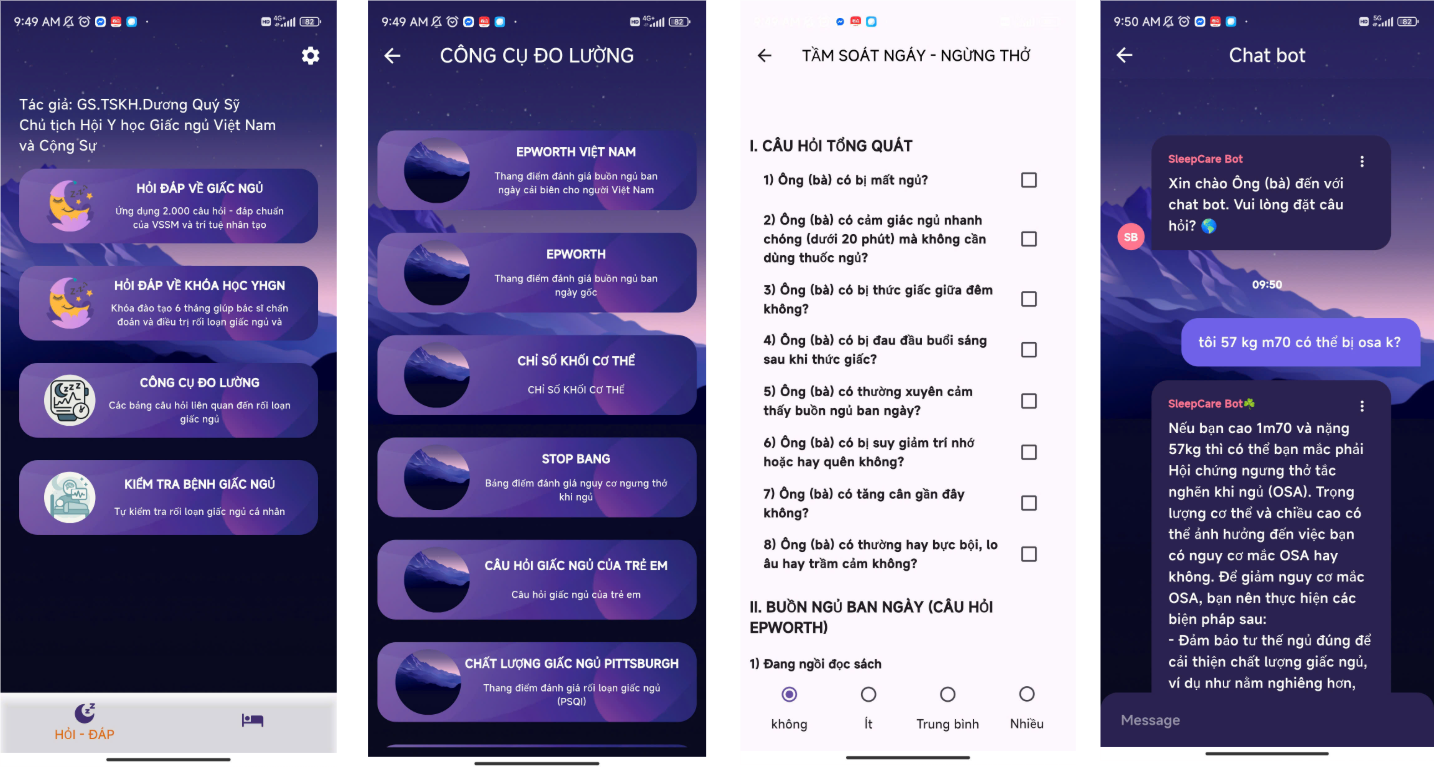
\includegraphics[width=0.8\linewidth]{images/appsleep.png}
    \caption{Giao diện chức năng chatbot và bộ câu hỏi tầm soát}
    \label{appsleep}
\end{figure}

\begin{lstlisting}[float,language=C,caption=Tập lệnh đánh giá tư thế ngủ bằng ngưỡng, label=nguong,captionpos=b]
static Function getPositionSleep = (double x, double y, double z) {
    if ((-6.5 < y && y < 6.5)) {
      if (-7.07 < x && x < 7.07) {
        if (z > 0) {
          return 1; // ngua
        }
        if (z < 0) {
          return 4; //sap
        }
      }
      if (x > 3) return 2; //trai
      if (x < -3) return 3; //phai
  }
    return 6; // khong phai nam
  };

\end{lstlisting}


Hình~\ref{appbieudo} minh họa giao diện hiển thị giá trị 
cảm biến theo thời gian thực. Phần đầu hiển thị biểu đồ ba trục 
x, y, z. Phần thứ hai là tổng thời gian theo từng tư thế ngủ 
được tính toán dựa trên tín hiệu nhận dạng. Phần cuối cùng cho biết 
tư thế hiện tại mà hệ thống đang xác định được. 
Tuy nhiên, phương pháp xác định tư thế dựa trên ngưỡng chưa có tính tổng quát cao. 
Do đó, trong các phần tiếp theo, các mô hình học máy sẽ 
được áp dụng để cải thiện độ chính xác và ổn định của hệ 
thống nhận diện tư thế. Việc cập nhật tư thế được thực hiện 
định kỳ mỗi 10 giây để tăng khả năng phản hồi theo thời gian thực.

\begin{figure}[htbp]
    \centering
    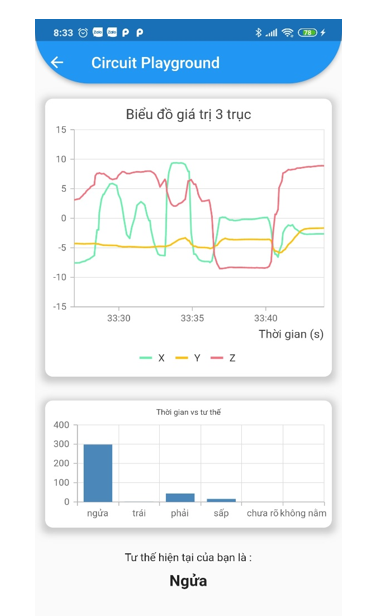
\includegraphics[width=0.3\linewidth]{images/appbieudo.png}
    \caption{Giao diện hiển thị dữ liệu gia tốc ba trục}
    \label{appbieudo}
\end{figure}

Về mặt kiến trúc lưu trữ dữ liệu, hệ thống được thiết kế phân tách 
giữa dữ liệu định tính và dữ liệu định lượng. Cụ thể, thông tin người 
dùng (tài khoản, cấu hình cá nhân), các bộ câu hỏi tầm soát 
(ví dụ: STOP-BANG, ESS), cùng với nội dung trả lời và phản hồi của 
chatbot được lưu trữ trong cơ sở dữ liệu quan hệ \textbf{PostgreSQL}. 
Cơ sở dữ liệu này hỗ trợ tính nhất quán cao và dễ dàng cho việc mở 
rộng truy vấn phức tạp trong các bài toán phân tích sau này.
Trong khi đó, dữ liệu cảm biến gia tốc được lưu trữ song song tại cơ 
sở dữ liệu phi quan hệ \textbf{MongoDB}, với định dạng BSON linh hoạt, 
phù hợp cho việc ghi nhận chuỗi thời gian lớn và truy xuất nhanh theo 
timestamp. Ngoài ra, hệ thống được mở rộng với các API cho phép trích 
xuất dữ liệu dưới dạng Excel, nhằm hỗ trợ phân tích và chia sẻ thông 
tin một cách linh hoạt.



\section{Thu thập và gắn nhãn dữ liệu}

\begin{figure}[htbp]
\centerline{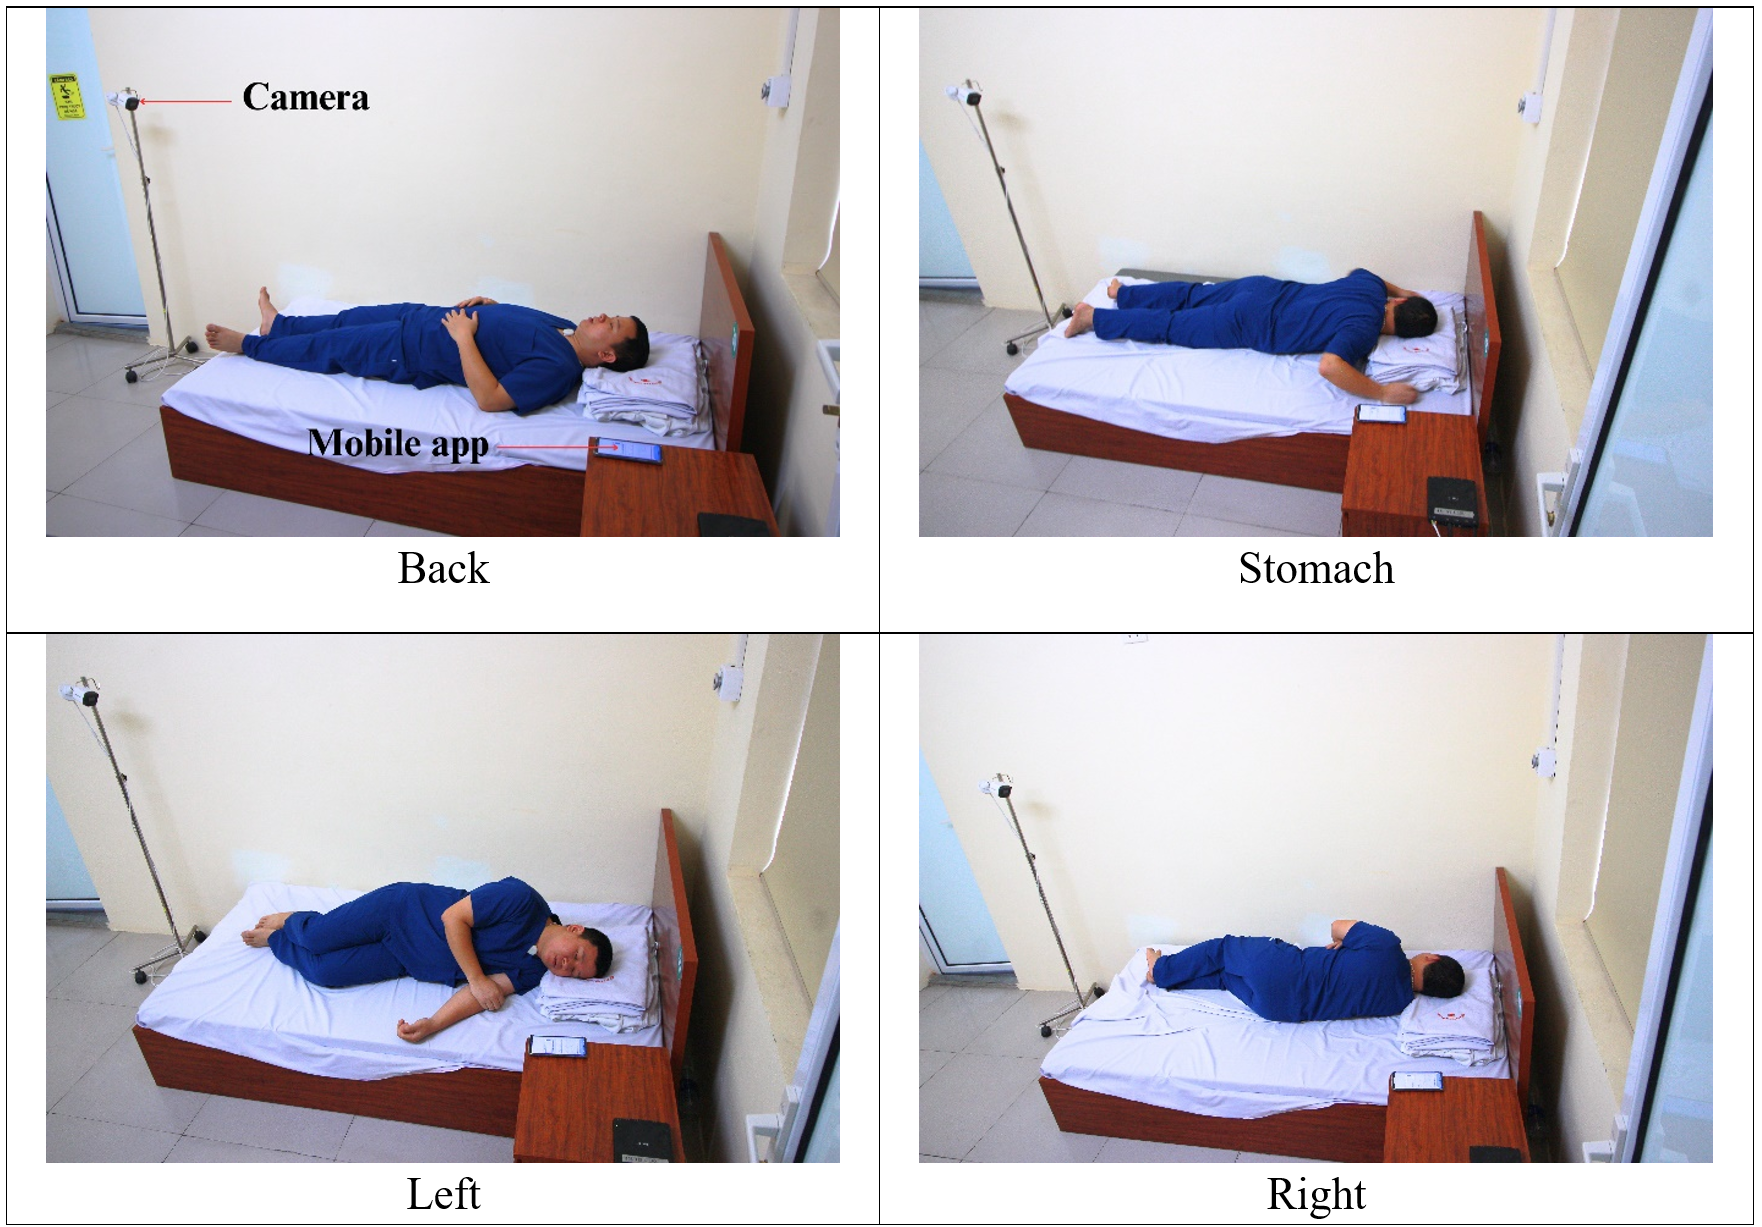
\includegraphics[width=0.8\linewidth]{images/4position.png}}
\caption{Mô phỏng thực nghiệm thực tế}
\label{4Position}
\end{figure}

Trong phần này, tác giả trình bày chi tiết phương pháp thu thập dữ liệu, 
các kịch bản thực nghiệm, cũng như quy trình xử lý và trích xuất đặc trưng 
để phục vụ cho việc huấn luyện các mô hình học máy trong bài toán nhận diện tư thế ngủ.

Tổng cộng 25 tình nguyện viên đã được tuyển chọn tham gia vào quá trình 
thu thập dữ liệu, với độ tuổi dao động từ 10 đến 60, trong đó độ tuổi 
phổ biến là 24. Nhóm tình nguyện viên bao gồm cả nam và nữ, được lựa 
chọn với tiêu chí đa dạng về giới tính và độ tuổi nhằm tăng tính đại 
diện và khách quan cho bộ dữ liệu.

Trong kịch bản đầu tiên (gọi là \textbf{thu thập có giám sát}), 
mỗi tình nguyện viên được hướng dẫn gắn thiết bị cảm biến vào vùng 
xương ức (ngay dưới hõm cổ) bằng băng keo y tế hai mặt 3M, 
sau đó đăng nhập vào ứng dụng di động với tài khoản cá nhân đã đăng ký. 
Dưới sự giám sát trực tiếp của tác giả, mỗi người tham gia sẽ lần 
lượt thực hiện các tư thế ngủ cơ bản (nằm ngửa, nằm sấp, nghiêng trái, nghiêng phải) 
trong thời gian tối thiểu 5 phút cho mỗi tư thế. 
Thứ tự thay đổi tư thế được thực hiện ngẫu nhiên nhằm tránh thiên 
lệch theo trình tự. Mỗi tư thế được lặp lại ít nhất hai lần để đảm 
bảo tính lặp lại và ổn định của tín hiệu.
Sau khi xác minh rằng dữ liệu cảm biến đã được lưu trữ đầy đủ 
trên hệ thống (kiểm tra trên MongoDB và giao diện ứng dụng), quá trình 
thu thập dữ liệu từ một tình nguyện viên được xem là hoàn tất.

Bên cạnh đó, để mô phỏng điều kiện thực tế khi sử dụng thiết bị trong 
sinh hoạt ban đêm, tác giả đã tự thực hiện kịch bản thứ hai 
(\textbf{thu thập trong giấc ngủ tự nhiên}). Trong kịch bản này, 
thiết bị được gắn vào cổ trước khi đi ngủ và ghi nhận dữ liệu liên 
tục trong suốt một đêm. Song song đó, một camera cố định được lắp 
đặt phía trên giường để ghi hình toàn bộ quá trình ngủ, từ đó hỗ 
trợ gán nhãn chính xác theo thời gian thực. Dữ liệu trong giai đoạn 
này được xử lý và đồng bộ thủ công giữa tín hiệu cảm biến và video 
để loại bỏ các đoạn có chuyển động hoặc sai lệch nhãn Hình~\ref{4Position}.

Mặc dù phương pháp thu thập trong môi trường tự nhiên sát với điều kiện 
sử dụng thực tế, nhưng đòi hỏi nhiều công sức xử lý hậu kỳ và 
khó kiểm soát chất lượng dữ liệu đầu vào. 
Theo ý kiến tư vấn từ các chuyên gia trong lĩnh vực y học giấc ngủ, 
phương pháp thu thập có giám sát (phương pháp 1) vẫn được ưu tiên do 
khả năng kiểm soát tốt, đảm bảo dữ liệu cân bằng giữa các tư thế, 
đồng thời vẫn duy trì được mức độ tương thích cao với điều kiện 
thực tế khi triển khai ứng dụng theo dõi tại nhà.

Sau quá trình thu thập, bộ dữ liệu huấn luyện bao gồm tổng cộng \textbf{158.750 mẫu} 
hợp lệ sau khi đã lọc nhiễu và loại bỏ các phiên ghi nhận không đạt yêu cầu của 25 tình nguyện viên. 
Dữ liệu kiểm thử sẽ là dữ liệu trong suốt một đêm ngủ tự nhiên của tác giả 
Việc gán nhãn dữ liệu được thực hiện thủ công bằng cách đồng bộ thời gian giữa 
tín hiệu cảm biến và dữ liệu video, sau đó loại bỏ toàn bộ các đoạn có chuyển động 
hoặc tư thế không rõ ràng. Kết quả là bộ dữ liệu kiểm thử gồm \textbf{64.258 mẫu} 
đảm bảo độ chính xác cao về mặt nhãn.

Tất cả dữ liệu thu thập từ các tình nguyện viên và tác giả đều được xuất ra định 
dạng \texttt{CSV}, bao gồm thông tin thời gian (timestamp), 
giá trị cảm biến trên ba trục $x$, $y$, $z$, và nhãn tư thế tương ứng 
(nếu có). Dữ liệu này được sử dụng làm đầu vào cho quá trình trích 
xuất đặc trưng và huấn luyện mô hình học máy.


\section{Phân loại tư thế ngủ bằng học máy}

\subsection{Phân tích dữ liệu}
Tư thế ngủ ban đầu có thể được ước lượng bằng phương pháp dựa trên ngưỡng 
(threshold-based), áp dụng trực tiếp lên dữ liệu cảm biến gia tốc ba 
trục. Trong phương pháp này, các ngưỡng được thiết lập trước cho từng 
trục ($x$, $y$, $z$), và sự thay đổi tư thế được suy đoán khi giá trị 
gia tốc đo được vượt quá ngưỡng tương ứng. Kỹ thuật này có ưu điểm là 
đơn giản, chi phí tính toán thấp, và đặc biệt phù hợp với các hệ thống 
nhúng tiêu thụ năng lượng thấp. 
Mặc dù kỹ thuật dựa trên ngưỡng có ưu điểm đơn giản và phù hợp với 
các hệ thống nhúng có tài nguyên hạn chế, nó tồn tại một số hạn chế 
nhất định. Cụ thể, phương pháp này khó phát hiện các chuyển động nhẹ 
hoặc tư thế trung gian giữa các trạng thái rõ ràng. Ngoài ra, các 
ngưỡng thường cần hiệu chỉnh theo từng cá nhân do sự khác biệt về 
hình thể, kiểu vận động và vị trí gắn cảm biến.


\begin{figure}[htbp]
\centering
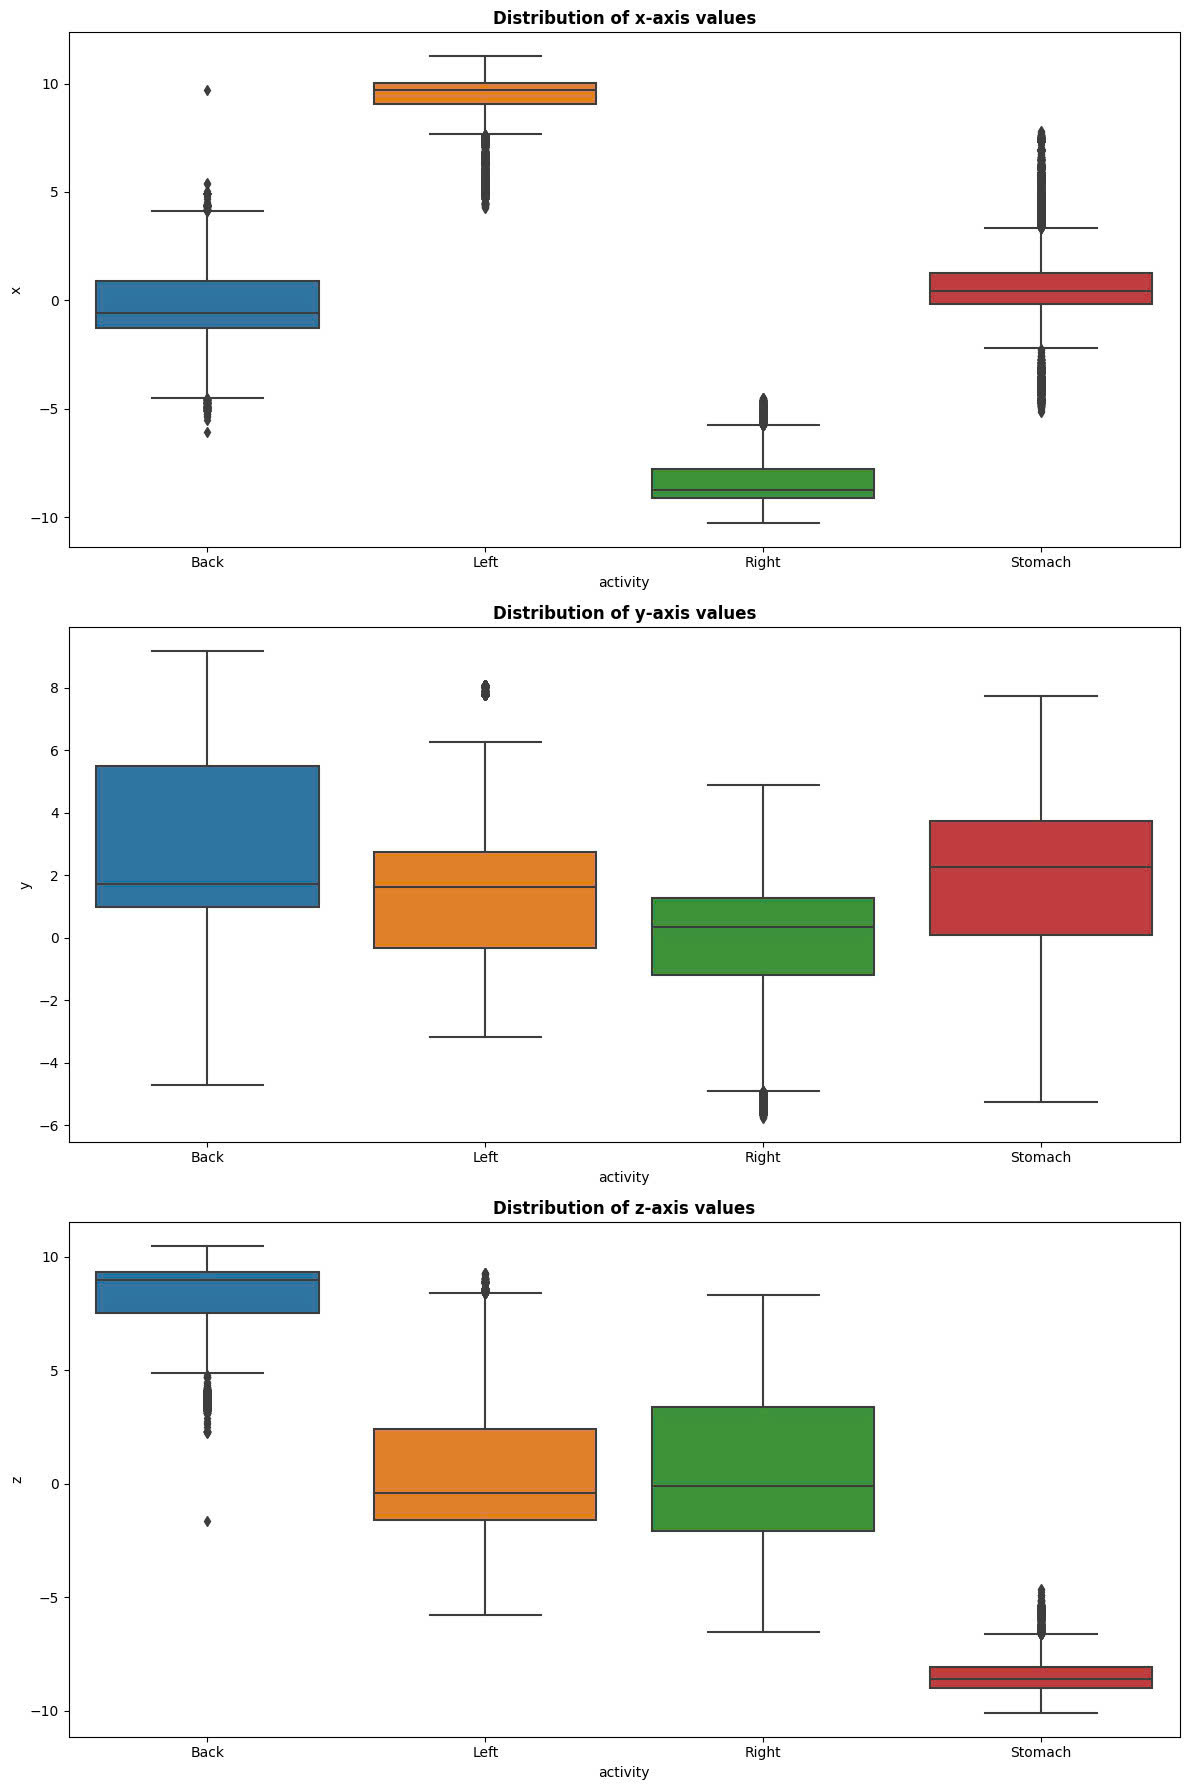
\includegraphics[width=0.7\linewidth]{images/threshhold.jpg} 
\caption{Phân bố dữ liệu cảm biến theo ba trục $x$, $y$, $z$ ứng với các tư thế ngủ khác nhau.}
\label{fig:axis_distribution}
\end{figure}
Hình~\ref{fig:axis_distribution} trình bày phân tích chi tiết phân bố 
tín hiệu cảm biến theo ba trục gia tốc ứng với bốn tư thế ngủ cơ bản. 
Ở trục $x$, các phân bố tương đối biệt lập, đặc biệt giữa hai tư thế 
nằm ngửa và nằm sấp, cũng như giữa nghiêng trái và nghiêng phải. 
Điều này cho thấy trục $x$ có khả năng phân biệt tư thế tốt. 
Ngược lại, trục $y$ thể hiện mức độ chồng lấn lớn giữa các tư thế, 
dẫn đến khả năng tách biệt thấp và ít giá trị trong việc xác định tư 
thế ngủ. Đối với trục $z$, có thể quan sát được sự phân tách 
rõ ràng giữa tư thế nằm nghiêng và các tư thế dọc 
(nằm ngửa và nằm sấp), chứng tỏ vai trò quan trọng của trục $z$ 
trong phân loại tư thế.



\begin{figure}[htbp]
\centering
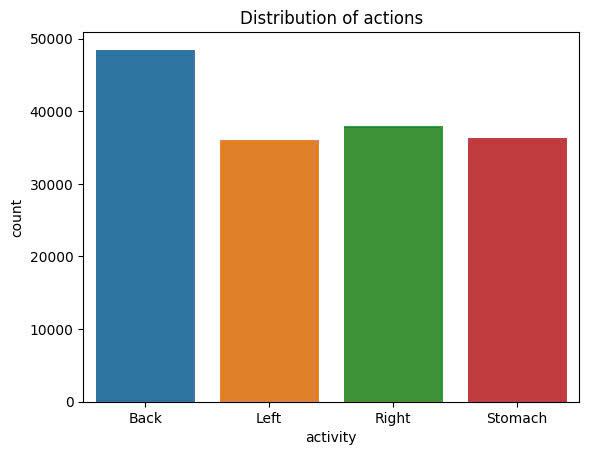
\includegraphics[width=0.6\linewidth]{images/distribution actions.jpg} 
\caption{Phân bố số lượng mẫu trong tập huấn luyện theo từng tư thế.}
\label{fig:countActions}
\end{figure}


Hình~\ref{fig:countActions} minh họa sự phân bố số lượng mẫu trong 
tập huấn luyện theo từng tư thế. Tư thế nằm ngửa (Back) chiếm tỷ 
trọng cao nhất với khoảng 50.000 mẫu, trong khi ba tư thế còn lại 
(nghiêng trái, nghiêng phải và nằm sấp) có số lượng tương đối cân bằng, 
dao động từ 30.000 đến 35.000 mẫu. Phân bố này phản ánh xu hướng phổ 
biến của tư thế nằm ngửa trong giấc ngủ tự nhiên, đồng thời cho thấy 
tầm quan trọng lâm sàng của tư thế này, đặc biệt trong bối cảnh hội 
chứng ngưng thở khi ngủ (OSA), khi tư thế nằm ngửa có thể làm trầm 
trọng tình trạng bệnh.



\subsection{Xử lý và trích xuất đặc trưng}

Dữ liệu cảm biến thu thập được trước tiên được xử lý khử nhiễu bằng 
phương pháp hiệu chỉnh điểm gốc (differential technique), bằng cách 
lấy hiệu giữa giá trị hiện tại và giá trị tham chiếu ban đầu trên ba 
trục $x$, $y$, và $z$. Sau đó, tín hiệu được chia thành các cửa sổ 
thời gian có độ dài 2 giây, với mức chồng lấn 50\% giữa các cửa sổ 
liên tiếp nhằm tăng độ mịn của chuỗi dữ liệu đầu vào.
Chỉ những cửa sổ dữ liệu có nhãn nhất quán trong toàn bộ thời gian 
mới được giữ lại để huấn luyện mô hình. Các cửa sổ chứa nhãn không 
đồng nhất (nhiều hơn một nhãn) hoặc có biểu hiện chuyển động bất 
thường sẽ bị loại bỏ khỏi quá trình xử lý tiếp theo.

\begin{table}[htbp]
\caption{Các đặc trưng thống kê và tín hiệu được sử dụng trong phân loại tư thế ngủ}
\label{tab:features}
\begin{center}
\renewcommand{\arraystretch}{1.5}
\begin{tabular}{|l|p{9.5cm}|}
\hline
\textbf{Đặc trưng} & \textbf{Mô tả / Công thức} \\
\hline
Giá trị trung bình & $\mu_s = \frac{1}{n} \sum_{i=1}^{n} S_i$ \\
\hline
Độ lệch chuẩn & $\sigma_s = \sqrt{\frac{1}{n} \sum_{i=1}^{n} (S_i - \mu_s)^2}$ \\
\hline
Độ lệch tuyệt đối trung bình & $\text{AAD} = \frac{1}{n} \sum_{i=1}^{n} |S_i - \mu_s|$ \\
\hline
Giá trị nhỏ nhất & $\min(s) = \min(S_1, S_2, \ldots, S_n)$ \\
\hline
Giá trị lớn nhất & $\max(s) = \max(S_1, S_2, \ldots, S_n)$ \\
\hline
Hiệu số lớn nhất - nhỏ nhất & $\max(s) - \min(s)$ \\
\hline
Trung vị & $\text{Median}(s) = \text{median}(S_1, S_2, \ldots, S_n)$ \\
\hline
Độ lệch tuyệt đối trung vị & $\text{MAD} = \frac{1}{n} \sum_{i=1}^{n} |S_i - \text{Median}(s)|$ \\
\hline
Khoảng tứ phân vị & $IQR = \text{percentile}(75) - \text{percentile}(25)$ \\
\hline
Số giá trị âm & $\#(S_i < 0)$ \\
\hline
Số giá trị dương & $\#(S_i > 0)$ \\
\hline
Số giá trị lớn hơn trung bình & $\#(S_i > \mu_s)$ \\
\hline
Số đỉnh (local maxima) & Số lượng điểm cực đại cục bộ trong chuỗi tín hiệu \\
\hline
Độ lệch (Skewness) & $\frac{1}{n \sigma_s^3} \sum_{i=1}^{n} (S_i - \mu_s)^3$ \\
\hline
Độ nhọn (Kurtosis) & $\frac{1}{n \sigma_s^4} \sum_{i=1}^{n} (S_i - \mu_s)^4$ \\
\hline
Năng lượng tín hiệu & $\sum_{i=1}^{n} S_i^2$ \\
\hline
Gia tốc tổng hợp trung bình & $\frac{1}{n} \sum_{i=1}^{n} \sqrt{x_i^2 + y_i^2 + z_i^2}$ \\
\hline
Tổng độ lớn tín hiệu (SMA) & $\frac{1}{n} \sum_{i=1}^{n} (|x_i| + |y_i| + |z_i|)$ \\
\hline
\end{tabular}
\end{center}
\end{table}

\subsubsection{Đặc trưng miền thời gian (T1)}\label{AA}

Dữ liệu cảm biến gia tốc vốn là chuỗi thời gian, do đó các đặc trưng miền thời gian đóng vai trò rất quan trọng trong nhận diện tư thế ngủ. Trong nghiên cứu này, tác giả trích xuất tổng cộng 40 đặc trưng thống kê cho mỗi cửa sổ dữ liệu, trên cả ba trục $x$, $y$, $z$. Các đặc trưng bao gồm giá trị trung bình, độ lệch chuẩn, độ lệch tuyệt đối trung bình, giá trị lớn nhất, nhỏ nhất, hiệu số lớn-nhỏ nhất, trung vị, độ lệch tuyệt đối trung vị, khoảng tứ phân vị, số lượng giá trị âm/dương, số lượng giá trị lớn hơn trung bình, số đỉnh tín hiệu, độ lệch, độ nhọn, năng lượng tín hiệu, gia tốc tổng hợp và tổng độ lớn tín hiệu. Các đặc trưng này được lựa chọn dựa trên tính dễ tính toán, hiệu quả phân tách tư thế và khả năng triển khai trên vi điều khiển.

\subsubsection{Đặc trưng miền tần số (F1)}\label{AA}

Để khai thác thông tin trong miền tần số, tác giả sử dụng Biến đổi Fourier Nhanh (FFT) để chuyển đổi dữ liệu từ miền thời gian sang miền tần số. Từ các cửa sổ tín hiệu sau biến đổi, 29 đặc trưng thống kê được tính toán, bao gồm các đặc trưng tương tự như trong miền thời gian: trung bình, độ lệch chuẩn, độ lệch tuyệt đối, giá trị cực đại – cực tiểu, trung vị, khoảng tứ phân vị, số đỉnh, độ lệch, độ nhọn, năng lượng tín hiệu,... Ngoài ra, hai đặc trưng kết hợp là gia tốc tổng hợp trung bình và tổng độ lớn tín hiệu (SMA) cũng được duy trì trong miền tần số để phục vụ so sánh với miền thời gian.

Việc sử dụng đồng thời các đặc trưng từ cả hai miền thời gian và tần số giúp tăng khả năng mô tả đặc trưng cho mô hình học máy, từ đó nâng cao hiệu quả phân loại tư thế ngủ trong các điều kiện khác nhau.

\subsection{Kịch bản kiểm thử và lựa chọn tính năng}

Lựa chọn đặc trưng là một bước quan trọng trong quá trình xây dựng mô hình học máy, giúp giảm chiều dữ liệu, cải thiện hiệu quả huấn luyện, rút ngắn thời gian tính toán và hạn chế hiện tượng quá khớp (overfitting). Nguyên lý chung là các đặc trưng hiệu quả phải có mối tương quan cao với biến mục tiêu (tư thế ngủ), đồng thời có mức tương quan thấp với nhau nhằm tránh dư thừa thông tin.

\textbf{Thứ nhất}, phân tích ma trận tương quan Pearson (Hình~\ref{fig:correlation}) đã cho thấy một số cặp đặc trưng có mức tương quan rất cao, điển hình như $x_{\mathrm{std}}$ và $x_{\mathrm{aad}}$ ($r = 0.98$), hay $y_{\mathrm{std}}$ và $y_{\mathrm{aad}}$ ($r = 0.68$). Điều này gợi ý rằng có thể loại bỏ một phần các đặc trưng trùng lặp nhằm giảm độ phức tạp mô hình mà vẫn giữ được thông tin cốt lõi.

\begin{figure}[htbp]
\centering
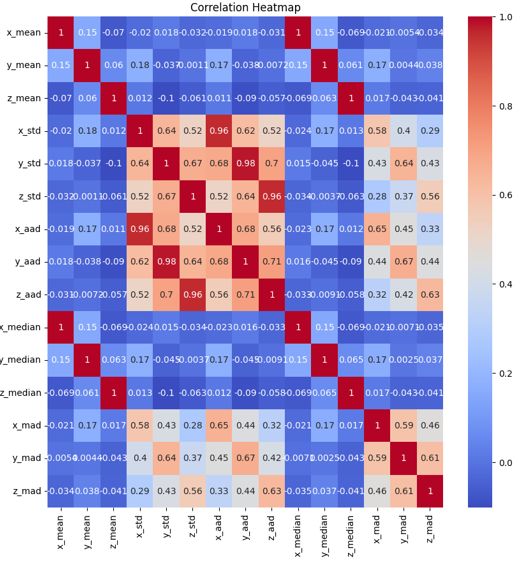
\includegraphics[width=1\linewidth]{images/correlation.png} 
\caption{Ma trận tương quan giữa các đặc trưng trích xuất. Cường độ màu thể hiện hệ số tương quan Pearson. Màu đỏ là tương quan dương mạnh, xanh là tương quan âm mạnh, xám là không tương quan.}
\label{fig:correlation}
\end{figure}

\textbf{Thứ hai}, kết quả phân tích SHAP (SHapley Additive exPlanations) ở Hình~\ref{fig:shap} chỉ ra rằng một số đặc trưng – đặc biệt là các đặc trưng miền thời gian trên trục $z$ như trung bình, năng lượng, trung vị – có ảnh hưởng vượt trội đến dự đoán của mô hình. Do đó, việc ưu tiên các đặc trưng này trong kịch bản triển khai nhẹ (TinyML) là hoàn toàn hợp lý về mặt kỹ thuật.

\begin{figure}[htbp]
\centering
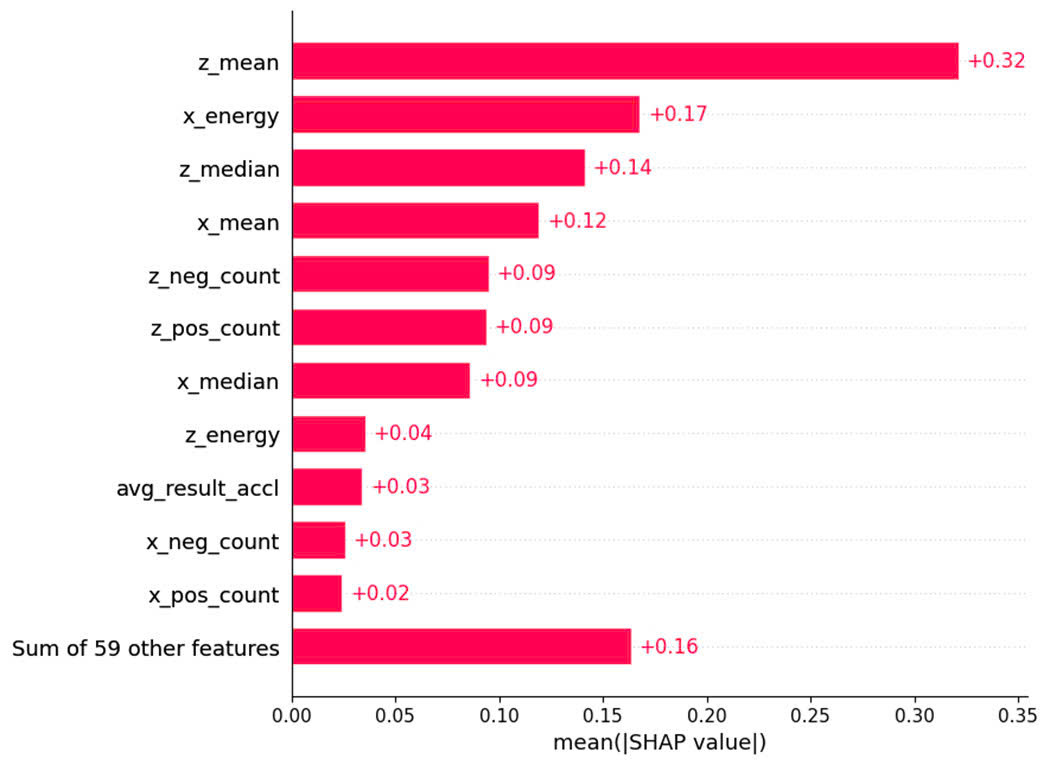
\includegraphics[width=0.8\linewidth]{images/shap20.jpg} 
\caption{Phân tích giá trị SHAP nhằm xác định tầm quan trọng của các đặc trưng trong mô hình phân loại tư thế ngủ. Các đặc trưng từ trục $z$ chiếm ưu thế về mức ảnh hưởng đến đầu ra mô hình.}
\label{fig:shap}
\end{figure}

\textbf{Thứ ba}, để hệ thống hóa việc đánh giá vai trò của từng nhóm đặc trưng và cấu hình mô hình, tác giả đã xây dựng tám kịch bản thực nghiệm được trình bày trong Bảng~\ref{tab:scenarios}. Các kịch bản được thiết kế nhằm phản ánh đầy đủ các yếu tố cần đánh giá như loại đặc trưng (miền thời gian, tần số), mức độ tương quan, độ dài cửa sổ tín hiệu và bộ đặc trưng tối ưu hoá bằng SHAP.

\begin{table}[htbp]
\caption{Các kịch bản lựa chọn và sử dụng đặc trưng trong nghiên cứu}
\label{tab:scenarios}
\begin{center}
\renewcommand{\arraystretch}{1.2}
\begin{tabular}{|c|p{6.1cm}|}
\hline
\textbf{Kịch bản} & \textbf{Mô tả} \\
\hline
1 & Sử dụng toàn bộ đặc trưng để đánh giá ảnh hưởng tổng thể đến mô hình. \\
\hline
2 & Áp dụng toàn bộ đặc trưng trong miền thời gian. \\
\hline
3 & Áp dụng toàn bộ đặc trưng trong miền tần số. \\
\hline
4 & Sử dụng đặc trưng miền thời gian, loại bỏ các đặc trưng có tương quan $>$ 95\%. \\
\hline
5 & Chọn ra 11 đặc trưng quan trọng nhất theo giá trị SHAP. \\
\hline
6 & Dùng cửa sổ 3 giây (50\% overlap), với 11 đặc trưng SHAP. \\
\hline
7 & Dùng cửa sổ 1 giây (50\% overlap), với 11 đặc trưng SHAP. \\
\hline
8 & Dùng cửa sổ 2 giây (25\% overlap), với 11 đặc trưng SHAP. \\
\hline
\end{tabular}
\end{center}
\end{table}

Đối với các kịch bản 5 đến 8, việc lựa chọn 11 đặc trưng được thực hiện bằng cách huấn luyện mô hình Random Forest trên toàn bộ tập đặc trưng, sau đó tính giá trị SHAP trung bình cho từng đặc trưng và chọn ra nhóm có ảnh hưởng cao nhất. Việc rút gọn đặc trưng này giúp mô hình nhẹ hơn, nhanh hơn, phù hợp với môi trường nhúng có giới hạn về bộ nhớ và tính toán.

Các kịch bản 6 đến 8 thay đổi độ dài cửa sổ trượt (1 giây, 2 giây, 3 giây) và mức chồng lấn nhằm khảo sát tác động của kích thước đoạn tín hiệu đến hiệu quả mô hình, đồng thời phản ánh điều kiện sử dụng thực tế trong các thiết bị đeo (wearables) hoặc hệ thống biên (edge-AI).

Với thiết kế kịch bản như trên, luận văn không chỉ đánh giá hiệu quả mô hình theo nhiều hướng khác nhau, mà còn hướng tới việc xác định cấu hình tối ưu giữa độ chính xác, chi phí tính toán và khả năng triển khai thực tiễn.

\subsection{Huấn luyện mô hình}

Dựa trên các phương pháp phân loại được đề cập ở các phần trước — 
bao gồm phương pháp ngưỡng, học máy và học sâu — 
tác giả đã lựa chọn một tập hợp đại diện các mô hình để 
tiến hành đánh giá hiệu quả trong bài toán nhận diện tư thế ngủ 
từ dữ liệu cảm biến gia tốc. Cụ thể, bốn mô hình học máy truyền 
thống được lựa chọn từ thư viện \texttt{scikit-learn} gồm: 
\textbf{Random Forest (RF)}, \textbf{Logistic Regression (LR)}, 
\textbf{Support Vector Machine (SVM)}, và \textbf{Gradient Boosting (GB)}. 
Đây đều là các mô hình đã được chứng minh hiệu quả trong việc xử lý dữ 
liệu cảm biến có cấu trúc, đặc biệt trong các bài toán phân loại đa lớp.

Để đảm bảo tính công bằng trong so sánh và khả năng triển khai thực tế trên vi điều khiển, các siêu tham số (hyperparameters) của từng mô hình được lựa chọn dựa trên kinh nghiệm thực tiễn trong các công trình trước và quá trình tinh chỉnh sơ bộ nhằm đạt được sự cân bằng giữa độ chính xác và độ phức tạp tính toán. Chi tiết tham số của từng mô hình được trình bày trong Bảng~\ref{tab:models}.

\begin{table}[htbp]
\caption{Các mô hình học máy và siêu tham số sử dụng trong nghiên cứu}
\label{tab:models}
\centering
\renewcommand{\arraystretch}{1.2}
\begin{tabular}{|l|p{9cm}|}
\hline
\textbf{Mô hình} & \textbf{Tham số cấu hình} \\
\hline
\textbf{Random Forest (RF)} & 
Số cây quyết định: 50; \newline
Độ sâu tối đa: 5; \newline
Số đặc trưng được xét tại mỗi nút: \texttt{log2} \\
\hline
\textbf{Logistic Regression (LR)} & 
Chiến lược đa lớp: \texttt{one-vs-rest}; \newline
Số vòng lặp tối đa: 50; \newline
Hàm tối ưu: \texttt{lbfgs} \\
\hline
\textbf{Support Vector Machine (SVM)} & 
Hàm kernel: \texttt{sigmoid}; \newline
Tham số điều chuẩn $C = 2$; \newline
Chiến lược đa lớp: \texttt{one-vs-rest} \\
\hline
\textbf{Gradient Boosting (GB)} & 
Tốc độ học: 0.01; \newline
Số lượng cây tăng cường: 50; \newline
Độ sâu tối đa: 3; \newline
Số đặc trưng được chọn: \texttt{log2} \\
\hline
\textbf{Mạng nơ-ron (Neural Network, Keras)} & 
Cấu trúc: [8, 4, \textit{num\_classes}]; \newline
Hàm kích hoạt: \texttt{ReLU}, \texttt{ReLU}, \texttt{Softmax}; \newline
Thuật toán tối ưu: \texttt{Adam} (learning rate = 0.01); \newline
Hàm mất mát: \texttt{sparse\_categorical\_crossentropy}; \newline
Độ đo đánh giá: \texttt{accuracy} \\
\hline
\end{tabular}
\end{table}

Ngoài các mô hình học máy, một mạng nơ-ron nhân tạo tuyến tính đơn giản 
(feedforward neural network) được xây dựng bằng thư viện \texttt{TensorFlow/Keras} 
để đại diện cho phương pháp học sâu. 
Mạng bao gồm hai lớp ẩn với số lượng nơ-ron lần lượt là 8 và 4, 
theo sau là một lớp đầu ra sử dụng hàm kích hoạt \texttt{Softmax} cho bài toán phân loại đa lớp. 
Các lớp ẩn sử dụng hàm kích hoạt \texttt{ReLU} nhằm mô hình hóa các quan hệ phi tuyến hiệu quả hơn. 
Mô hình này được tối ưu bằng thuật toán \texttt{Adam} với tốc độ học (learning rate) là 0.01 
và được huấn luyện bằng hàm mất mát \texttt{sparse\_categorical\_crossentropy}, 
sử dụng độ đo đánh giá \texttt{accuracy} để phản ánh hiệu suất phân loại.

Việc lựa chọn kết hợp các mô hình với mức độ phức tạp khác nhau cho phép đánh giá toàn diện về 
hiệu quả phân loại trong các điều kiện thực tế. 
Từ các mô hình cây đơn giản và dễ diễn giải, đến các mô hình mạnh 
hơn như Gradient Boosting hoặc mạng nơ-ron – nghiên cứu nhằm tìm r
a giải pháp cân bằng tối ưu giữa độ chính xác, kích thước mô hình, 
tốc độ suy luận (inference latency) và mức sử dụng bộ nhớ, 
phục vụ cho các ứng dụng thực tiễn như hệ thống AI biên (Edge-AI) 
hoặc thiết bị đeo thông minh.
\subsection{Đánh giá kết quả}
Để đánh giá hiệu quả của các mô hình học máy và tác động của lựa 
chọn đặc trưng đầu vào, tám kịch bản thực nghiệm đã được thiết kế 
như trình bày ở các phần trước. Các kịch bản này không chỉ cho phép 
phân tích ảnh hưởng của đặc trưng, cửa sổ tín hiệu và trục cảm biến, 
mà còn hướng đến tối ưu hóa trọng số mô hình phục vụ triển khai trên 
thiết bị nhúng.


\begin{table}[htbp]
\caption{Độ chính xác phân loại của các mô hình trong 8 kịch bản}
\label{tab:accuracy}
\centering
\renewcommand{\arraystretch}{1.1}
\scriptsize
\begin{tabular}{|l|c|c|c|c|c|c|c|c|}
\hline
\textbf{Mô hình} & S1 & S2 & S3 & S4 & S5 & S6 & S7 & S8 \\
\hline
LR  & 0.970 & 0.970 & 0.368 & 0.970 & 0.987 & 0.990 & 0.990 & 0.987 \\
RF  & 0.995 & 0.996 & 0.426 & 0.994 & 0.993 & 0.993 & 0.993 & 0.991 \\
SVM & 0.995 & 0.985 & 0.280 & 0.991 & 0.989 & 0.982 & 0.982 & 0.870 \\
GB  & 0.996 & 0.996 & 0.439 & 0.995 & 0.995 & 0.996 & 0.996 & 0.996 \\
NN  &  0.920 &  --   &  --   &  --   &  --   &  --   &  --   & -- \\
\hline
\end{tabular}
\end{table}

Kết quả trong Bảng~\ref{tab:accuracy} làm sáng tỏ sự khác biệt căn bản giữa các nhóm đặc trưng và cách tiếp cận mô hình. 
Trước hết, \textbf{Gradient Boosting (GB)} nổi bật với hiệu năng ổn định nhất, 
liên tục đạt giá trị chính xác tối đa (0.996) trong năm kịch bản (S1, S2, S6, S7, S8). 
Đặc điểm này cho thấy ưu thế vượt trội của các phương pháp tăng cường mô hình dựa trên cây quyết định, 
khả năng khai thác tốt cả quan hệ phi tuyến và sự tương tác giữa các đặc trưng. 
\textbf{Random Forest (RF)} mặc dù có đôi chút biến thiên, nhưng vẫn duy trì độ chính xác vượt ngưỡng 0.99 trong hầu hết kịch bản, 
củng cố vai trò của các mô hình ensemble dựa trên bootstrap aggregation trong việc giảm phương sai và cải thiện khả năng tổng quát hoá.  

Trái lại, \textbf{Logistic Regression (LR)} và \textbf{Support Vector Machine (SVM)} 
chỉ đạt được hiệu năng tiệm cận 0.99 trong các kịch bản sử dụng đặc trưng miền thời gian hoặc đặc trưng được lựa chọn bằng SHAP. 
Đặc biệt, ở kịch bản S3 – vốn chỉ khai thác đặc trưng miền tần số – cả hai mô hình này sụt giảm nghiêm trọng về độ chính xác (LR còn 0.368, SVM chỉ 0.280). 
Kết quả nhấn mạnh rằng các tín hiệu động học quan trọng để phân loại chủ yếu được mã hoá trong miền thời gian. 
Điều này hoàn toàn tương thích với phân tích SHAP (Hình~\ref{fig:shap}), 
khi các đặc trưng đóng góp nhiều nhất đều tập trung ở miền thời gian, đặc biệt trên trục $z$, 
nơi thể hiện rõ sự khác biệt về động học tư thế.

Một điểm đáng chú ý khác là khi áp dụng cơ chế chọn lọc đặc trưng dựa trên \textbf{SHAP} (các kịch bản S5–S8), 
độ chính xác của các mô hình hầu như không suy giảm, thậm chí trong một số trường hợp còn được cải thiện nhẹ 
(ví dụ LR đạt 0.990 ở S6 và S7 so với 0.970 ở S1). 
Điều này chứng tỏ việc loại bỏ các đặc trưng dư thừa và tập trung vào những đặc trưng quan trọng nhất 
không chỉ giúp giảm chiều dữ liệu mà còn hạn chế hiện tượng nhiễu, từ đó gia tăng độ khái quát hoá. 
Kết quả này có ý nghĩa thực tiễn quan trọng, vì nó cho phép duy trì hiệu năng phân loại cao 
trong khi giảm thiểu chi phí tính toán và bộ nhớ – yếu tố then chốt khi triển khai trên các thiết bị nhúng hoặc hệ thống IoT có tài nguyên hạn chế.

Tóm lại, Bảng~\ref{tab:accuracy} không chỉ xác nhận ưu thế vượt trội của các mô hình ensemble như GB và RF, 
mà còn chứng minh tính hiệu quả của phương pháp chọn lọc đặc trưng dựa trên SHAP. 
Sự thất bại rõ rệt của kịch bản S3 nhấn mạnh rằng miền tần số không mang lại giá trị phân loại đáng kể trong trường hợp này, 
trong khi các đặc trưng miền thời gian mới là nguồn thông tin then chốt để mô hình học được ranh giới phân lớp một cách chính xác và bền vững.




\begin{figure}[htbp]
    \centering
    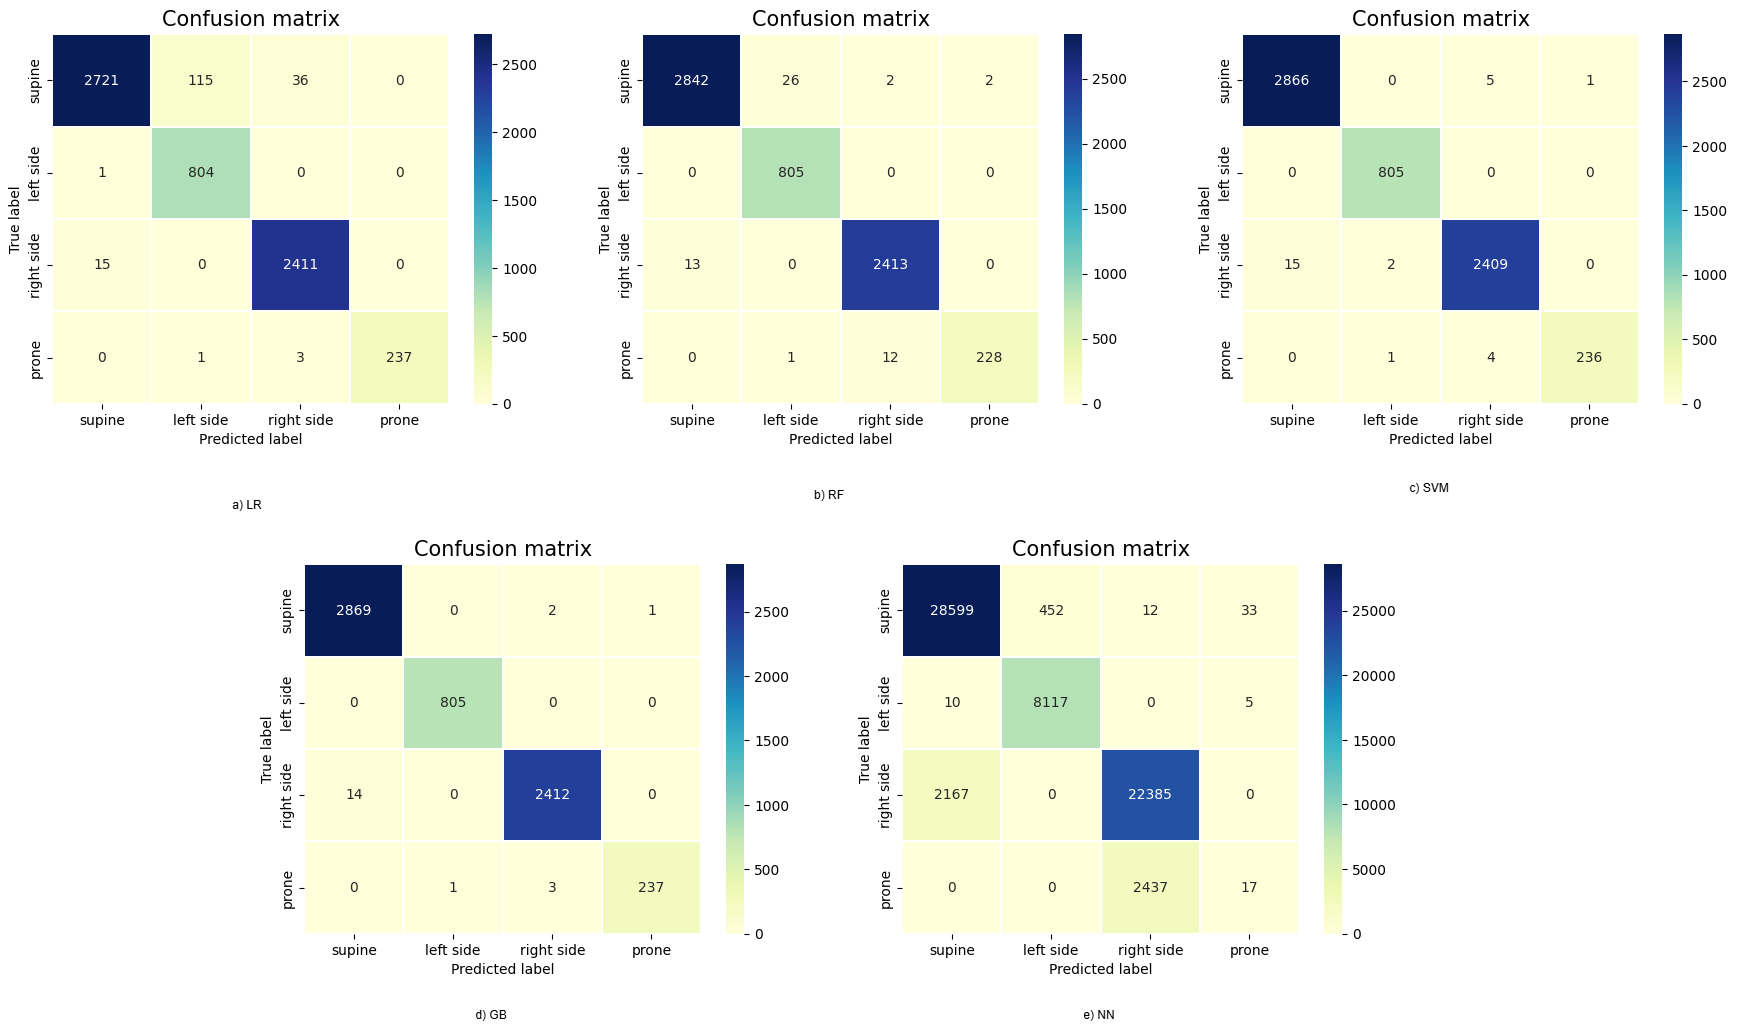
\includegraphics[width=\linewidth]{images/matrix (2).png}
    \caption{Ma trận nhầm lẫn (confusion matrix) của năm mô hình 
    phân loại trong kịch bản S1. GB và RF cho kết quả chính xác 
    cao nhất. Mô hình NN được huấn luyện trực tiếp trên dữ liệu thô.}
    \label{fig:cm_all_models}
\end{figure}

Kết quả này nhấn mạnh vai trò then chốt của lựa chọn đặc trưng đầu vào đối với hiệu quả mô hình. Các kịch bản sử dụng đặc trưng đã rút gọn theo SHAP (như S5–S8) vừa đạt độ chính xác cao, vừa giảm số chiều dữ liệu đầu vào, qua đó hỗ trợ triển khai mô hình nhẹ trong môi trường nhúng. Ngược lại, các kịch bản thiếu chọn lọc như S3 dẫn đến hiệu suất kém.

\begin{table}[htbp]
\caption{Kích thước mô hình (KB) trong 8 kịch bản}
\label{tab:modelsize}
\centering
\renewcommand{\arraystretch}{1.1}
\scriptsize
\begin{tabular}{|l|c|c|c|c|c|c|c|c|}
\hline
\textbf{Mô hình} & S1 & S2 & S3 & S4 & S5 & S6 & S7 & S8 \\
\hline
LR  & 4   & 2   & 2    & 2   & 2   & 2   & 2   & 2   \\
RF  & 187 & 151 & 291  & 176 & 89  & 89  & 141 & 103 \\
SVM & 315 & 232 & 3051 & 294 & 150 & 92  & 183 & 274 \\
GB  & 605 & 602 & 615  & 603 & 587 & 587 & 587 & 589 \\
NN  & 55  & --  & --   & --  & --  & --  & --  & --   \\
\hline
\end{tabular}
\end{table}

Bảng~\ref{tab:modelsize} cho thấy sự khác biệt đáng kể về kích thước giữa các mô hình. 
\textbf{Gradient Boosting (GB)} luôn duy trì dung lượng trên 580~KB bất kể kịch bản, 
cho thấy tính ổn định nhưng đồng thời cũng phản ánh hạn chế khi triển khai trên thiết bị nhúng có bộ nhớ giới hạn. 
\textbf{Random Forest (RF)} có kích thước biến thiên rõ rệt (89–291~KB) phụ thuộc vào số lượng và loại đặc trưng đầu vào, 
song vẫn duy trì ở mức chấp nhận được đối với các nền tảng nhúng có tài nguyên trung bình.  

Ngược lại, \textbf{Logistic Regression (LR)} chỉ chiếm 2–4~KB, 
một dung lượng cực kỳ nhỏ, khiến mô hình này trở thành ứng viên lý tưởng trong các hệ thống vi điều khiển hoặc IoT cần tối ưu bộ nhớ, 
mặc dù độ chính xác có phần thấp hơn so với các mô hình ensemble. 
\textbf{Support Vector Machine (SVM)} thường dao động trong khoảng 92–315~KB, 
tuy nhiên ở kịch bản S3 kích thước tăng vọt lên 3051~KB, 
nguyên nhân xuất phát từ số chiều đầu vào lớn và cấu trúc bộ nhớ của kernel. 
Điều này cho thấy SVM kém ổn định về mặt tài nguyên và khó kiểm soát khi triển khai thực tế.  

Đáng chú ý, \textbf{Neural Network (NN)} ở kịch bản S1 đạt độ chính xác 0.92 với dung lượng chỉ 55~KB. 
Mặc dù chưa đạt hiệu năng tối ưu, kết quả này mở ra hướng tiếp cận tiềm năng cho các ứng dụng Edge AI, 
nơi sự cân bằng giữa hiệu năng và tính gọn nhẹ được đặt lên hàng đầu.  

Tổng thể, Bảng~\ref{tab:modelsize} nhấn mạnh bài toán đánh đổi (trade-off) giữa \emph{hiệu quả dự đoán} và \emph{tài nguyên triển khai}. 
Trong khi RF và GB cho kết quả phân loại vượt trội về độ chính xác, 
thì LR và NN lại nổi bật nhờ kích thước gọn nhẹ, đặc biệt phù hợp với môi trường hạn chế tài nguyên. 
Sự đánh đổi này cho thấy rằng lựa chọn mô hình tối ưu không chỉ dựa vào độ chính xác thuần tuý, 
mà còn phụ thuộc vào yêu cầu hệ thống và ngữ cảnh triển khai cụ thể.
Từ hai bảng kết quả có thể thấy rõ sự đánh đổi giữa \emph{hiệu năng phân loại} và \emph{tài nguyên triển khai}. 
Trong bối cảnh nghiên cứu hướng đến ứng dụng trên thiết bị nhúng và hệ thống IoT, 
các mô hình có kích thước gọn nhẹ nhưng vẫn duy trì độ chính xác ở mức cao cần được ưu tiên. 
Do đó, mặc dù \textbf{RF} và \textbf{GB} thể hiện hiệu năng vượt trội về mặt độ chính xác, 
luận án lựa chọn thử nghiệm chuyên sâu với \textbf{Logistic Regression (LR)} và \textbf{Neural Network (NN)}. 
Hai mô hình này có ưu điểm quan trọng: dung lượng bộ nhớ rất nhỏ (2--4~KB đối với LR, 55~KB đối với NN) 
và khả năng triển khai thuận lợi trên vi điều khiển, vốn thường chỉ có vài trăm kilobyte bộ nhớ khả dụng.  

Một điểm cần lưu ý là các kịch bản S1–S5 được xây dựng với cửa sổ trượt 2~giây, 
trong khi các kịch bản S7 sử dụng cửa sổ 1~giây với mức chồng lấn 50\%. 
Kết quả cho thấy việc giảm độ dài cửa sổ từ 2~giây xuống 1~giây không làm suy giảm đáng kể độ chính xác 
(thậm chí trong một số trường hợp, LR và GB còn cải thiện nhẹ, ví dụ LR đạt 0.990 ở S7 so với 0.987 ở S5). 
Việc lựa chọn cửa sổ 1~giây thay vì 2~giây có ý nghĩa thực tiễn quan trọng: 
nó cho phép hệ thống phản hồi nhanh hơn, nắm bắt kịp thời sự thay đổi tư thế, 
đồng thời giảm độ trễ trong nhận dạng – một yêu cầu thiết yếu khi triển khai trong môi trường y tế thực tế.  

Tóm lại, mặc dù các mô hình ensemble như RF và GB đạt hiệu năng cao nhất về mặt số liệu, 
luận án định hướng ưu tiên triển khai thử nghiệm với LR và NN kết hợp cửa sổ 1~giây. 
Đây là lựa chọn cân bằng hợp lý giữa \emph{độ chính xác}, \emph{tính gọn nhẹ của mô hình}, 
và \emph{khả năng đáp ứng thời gian thực} khi triển khai trong các hệ thống nhúng hỗ trợ giám sát sức khỏe.

\section{Triển khai trên vi điều khiển nhúng}

Sau khi hoàn tất quá trình huấn luyện và đánh giá trên máy tính, bước tiếp theo của nghiên cứu là kiểm chứng khả năng triển khai mô hình trong môi trường thực tế sử dụng vi điều khiển nhúng. Mục tiêu khoa học ở giai đoạn này không chỉ dừng ở việc “chạy được” mô hình trên phần cứng hạn chế, mà còn nhằm làm sáng tỏ mối quan hệ đánh đổi giữa hiệu năng thuật toán và giới hạn tài nguyên của hệ thống nhúng.  

Cụ thể, nghiên cứu tiến hành triển khai song song hai mô hình: mạng nơ-ron nông (Neural Network – NN) với khả năng biểu diễn phi tuyến mạnh mẽ, và hồi quy logistic (Logistic Regression – LR) với cấu trúc tuyến tính cực kỳ gọn nhẹ. NN được kỳ vọng duy trì độ chính xác cao trong phân loại tư thế ngủ, trong khi LR đóng vai trò như một đối chứng quan trọng, minh chứng cho khả năng đạt được sự cân bằng tối ưu giữa độ chính xác vừa đủ và mức tiêu thụ tài nguyên tối thiểu.  

Điều này cho thấy trong bối cảnh phần cứng hạn chế, giá trị khoa học không nằm ở việc đạt độ chính xác tuyệt đối trong điều kiện lý tưởng, mà ở khả năng thiết kế một mô hình “đủ tốt” nhưng có thể vận hành bền vững trên chip. Chính sự đánh đổi này khẳng định nguyên lý cốt lõi của TinyML: hy sinh một phần nhỏ về độ chính xác để đổi lấy tính khả thi, hiệu quả năng lượng và độ tin cậy trong môi trường thực.  

Kết quả cũng cho thấy sự song hành giữa hai mô hình được lựa chọn. Mạng nơ-ron (NN) duy trì độ chính xác cao nhưng tiêu tốn nhiều tài nguyên, trong khi hồi quy logistic (LR) có dung lượng siêu nhỏ, tốc độ suy luận nhanh, và vẫn giữ mức chính xác tiệm cận. Việc triển khai song song cả NN và LR trên chip vì vậy không chỉ mang ý nghĩa kiểm chứng kỹ thuật, mà còn cung cấp bằng chứng khoa học cho thấy ranh giới cân bằng giữa “độ chính xác tối đa” và “khả năng ứng dụng thực tế” trong hệ thống nhúng y sinh.


\subsection{Quy trình triển khai mô hình}


Dựa trên các kết quả phân tích và đánh giá ở giai đoạn~1, 
tác giả quyết định bước sang giai đoạn~2 với mục tiêu triển khai thực tế trên phần cứng nhúng. 
Như đã trình bày, hai mô hình được lựa chọn cho thử nghiệm là \textbf{Neural Network (NN)} 
và \textbf{Logistic Regression (LR)}, bởi chúng đáp ứng tốt yêu cầu về tính gọn nhẹ và khả năng triển khai trên vi điều khiển.  

Quy trình triển khai bao gồm các bước sau:  
\begin{enumerate}
    \item \textbf{Xác định vi điều khiển mục tiêu}: lựa chọn nền tảng phần cứng phù hợp với giới hạn bộ nhớ và khả năng tính toán.  
    \item \textbf{Thu thập lại dữ liệu trực tiếp trên vi điều khiển}: đảm bảo dữ liệu phản ánh đúng điều kiện hoạt động của phần cứng thực tế, tránh sai lệch do khác biệt môi trường so với giai đoạn mô phỏng.  
    \item \textbf{Huấn luyện lại mô hình}: sử dụng bộ dữ liệu thu thập mới để tinh chỉnh và tái huấn luyện, nhằm tối ưu hóa mô hình cho nền tảng phần cứng được chọn.  
    \item \textbf{Chuyển đổi mô hình sang mã C/C++}: áp dụng các công cụ biên dịch và chuyển đổi chuyên dụng để xuất mô hình dưới dạng mã nguồn có thể nhúng trực tiếp.  
    \item \textbf{Triển khai trên chip}: nạp mã nguồn vào vi điều khiển, bộ lọc, kiểm tra khả năng suy luận và hiệu năng thời gian thực.  
\end{enumerate}

Vi điều khiển được lựa chọn là \textbf{Arduino Nano 33 BLE Sense}, sử dụng chip \texttt{nRF52840} (ARM Cortex-M4F, 64~MHz), 1~MB flash và 256~KB RAM. Bo mạch này cũng tích hợp sẵn cảm biến gia tốc, rất phù hợp để xây dựng hệ thống nhận diện tư thế ngủ hoàn chỉnh và hoạt động độc lập.


Qua nhiều lần triển khai thực nghiệm trực tiếp trên vi điều khiển, 
tác giả đã rút ra một kết luận quan trọng: 
việc \textbf{giảm số lượng mẫu huấn luyện} kết hợp với \textbf{rút gọn tập đặc trưng} 
mang lại hiệu quả rõ rệt trong việc tối ưu mô hình cho môi trường nhúng. 
Cụ thể, các mô hình sau khi được tinh giản có \emph{kích thước tệp nhỏ hơn}, 
\emph{mức sử dụng bộ nhớ giảm đáng kể}, và \emph{thời gian suy luận nhanh hơn}, 
nhưng độ chính xác chỉ suy giảm ở mức rất nhỏ và hoàn toàn nằm trong ngưỡng chấp nhận được đối với ứng dụng thực tế. 
Điều này chứng tỏ rằng, trong bối cảnh triển khai Edge AI, 
sự đánh đổi giữa số lượng đặc trưng và hiệu năng mô hình có thể được cân bằng một cách hợp lý, 
từ đó vừa đảm bảo tính khả thi trên phần cứng hạn chế, vừa duy trì độ tin cậy trong dự đoán.  

Đặc biệt, ở \textbf{bước 2 của quy trình}, tác giả đã tiến hành \emph{thu thập lại 10.430 mẫu dữ liệu} 
trực tiếp từ thiết bị \textbf{Arduino Nano 33 BLE Sense}. 
Khác với bộ dữ liệu mô phỏng trên máy tính, tập dữ liệu này phản ánh sát thực tế điều kiện hoạt động của phần cứng, 
bao gồm cả đặc điểm nhiễu, độ trễ và sai số phép đo. 
Nhờ vậy, việc huấn luyện lại mô hình trên tập dữ liệu thực nghiệm giúp tăng tính tương thích giữa mô hình và nền tảng nhúng, 
giảm thiểu nguy cơ sai lệch do khoảng cách giữa môi trường mô phỏng và môi trường thực thi.  

Trong quá trình triển khai thực tế, tác giả tiến hành hai hướng tiếp cận riêng biệt 
tương ứng với hai mô hình đã được lựa chọn từ giai đoạn~1: \textbf{Logistic Regression (LR)} và \textbf{Neural Network (NN)}.  

\begin{itemize}
    \item \textbf{Đối với LR:} sau khi huấn luyện lại mô hình trên tập dữ liệu thu thập từ Arduino Nano 33, 
    toàn bộ tham số bao gồm trọng số, hệ số bias và giá trị chuẩn hoá (min, max, scale) 
    được xuất trực tiếp sang mã C/C++. Cách tiếp cận này cho phép mô hình LR 
    được biểu diễn dưới dạng các mảng hằng số \texttt{const float[]} trong chương trình Arduino, 
    từ đó vi điều khiển có thể tính toán đầu ra bằng phép nhân ma trận và cộng bias đơn giản. 
    Việc xuất mô hình theo phương thức này đảm bảo kích thước file rất nhỏ (chỉ vài kilobyte) 
    và suy luận có thể thực hiện nhanh chóng mà không phụ thuộc vào thư viện học máy phức tạp.  

    \item \textbf{Đối với NN:} mô hình được thiết kế với hai lớp ẩn (8 và 4 nơ-ron), 
    sử dụng hàm kích hoạt ReLU và lớp đầu ra Softmax. Sau khi huấn luyện, 
    mô hình được chuyển đổi sang định dạng \textbf{TensorFlow Lite (TFLite)} bằng công cụ \texttt{TFLiteConverter}. 
    File nhị phân \texttt{.tflite} sau đó được ánh xạ sang mã C thông qua tiện ích \texttt{xxd -i}, 
    tạo thành một mảng byte \texttt{const unsigned char[]} để nạp trực tiếp vào bộ nhớ của vi điều khiển. 
    Cách tiếp cận này cho phép duy trì toàn bộ cấu trúc của mạng nơ-ron, 
    đồng thời tận dụng khả năng tối ưu hoá suy luận của TensorFlow Lite trên nền tảng nhúng.  
\end{itemize}

Sự khác biệt giữa hai phương pháp này phản ánh bản chất của từng mô hình: 
LR dựa trên phương trình tuyến tính với đặc trưng đã trích xuất, 
nên việc chuyển đổi tham số sang C/C++ là tối ưu và gọn nhẹ nhất. 
Ngược lại, NN có cấu trúc phi tuyến và nhiều lớp, do đó cần sử dụng định dạng TFLite 
để đóng gói toàn bộ mô hình dưới dạng nhị phân, vừa đảm bảo tính toàn vẹn, 
vừa khai thác được khả năng tối ưu hoá suy luận trên chip.  

Qua đó, luận án đã thiết lập được hai quy trình triển khai hoàn chỉnh:  
(i) LR với mô hình tuyến tính tối giản, phù hợp với các hệ thống nhúng cực kỳ hạn chế tài nguyên;  
(ii) NN với mô hình phi tuyến phức tạp hơn, tận dụng TFLite để cân bằng giữa độ chính xác và tốc độ suy luận.  

Trong bước triển khai thực tế, mô hình Logistic Regression (LR) được ánh xạ trực tiếp sang mã C/C++ 
thông qua ba thành phần chính: (i) tệp \texttt{model.h} lưu trữ toàn bộ tham số huấn luyện (trọng số, hệ số bias, 
giá trị chuẩn hoá); (ii) tệp \texttt{predict.h} định nghĩa cơ chế suy luận bằng phép tính tuyến tính kết hợp Softmax; 
và (iii) chương trình chính điều khiển cảm biến, trích xuất đặc trưng, chuẩn hoá và gọi hàm dự đoán. 
Cách tổ chức này giúp mô hình hoạt động độc lập hoàn toàn trên vi điều khiển mà không cần bất kỳ thư viện học máy ngoài nào.  

Thực nghiệm cho thấy toàn bộ quá trình suy luận được thực hiện chỉ với các phép toán cơ bản 
(\emph{cộng, nhân, căn bậc hai, hàm mũ}), tiêu tốn rất ít tài nguyên tính toán 
và đạt thời gian xử lý ở mức micro giây cho mỗi cửa sổ dữ liệu. 
Điều này khẳng định tính phù hợp của LR trong bối cảnh triển khai trên thiết bị nhúng 
có bộ nhớ và công suất xử lý hạn chế.  

Từ góc độ khoa học, việc triển khai LR theo cách này minh chứng rằng một mô hình học máy 
có thể được rút gọn thành tập tham số tĩnh và tái hiện chính xác trên chip, 
đồng thời duy trì độ chính xác ở mức chấp nhận được cho ứng dụng giám sát sức khoẻ thời gian thực. 
Chiến lược \textbf{tối giản mô hình} này là minh chứng rõ rệt cho tính khả thi của Edge AI: 
đảm bảo độ trễ thấp, tính riêng tư dữ liệu và khả năng vận hành bền vững trong môi trường hạn chế tài nguyên.

Khác với LR, mô hình Neural Network (NN) được triển khai trên chip thông qua định dạng 
\textbf{TensorFlow Lite Micro (TFLM)}. Sau khi huấn luyện, mô hình Keras được chuyển đổi sang 
tệp nhị phân \texttt{.tflite} và sau đó nhúng trực tiếp vào chương trình Arduino dưới dạng mảng byte 
(\texttt{const unsigned char model[]}). Việc này cho phép vi điều khiển thực thi suy luận với sự hỗ trợ 
của thư viện TFLM, vốn đã được tối ưu hóa cho các hệ thống nhúng có bộ nhớ giới hạn.  

Trong chương trình triển khai, bộ gia tốc của Arduino Nano 33 BLE Sense 
cung cấp dữ liệu ba trục $(x, y, z)$ liên tục. Tiếp đó dữ liệu được chuẩn hóa để bảo đảm sự tương thích với dải giá trị đầu vào mà mô hình đã được huấn luyện.  

Khối \texttt{MicroInterpreter} trong TFLM chịu trách nhiệm phân bổ bộ nhớ, 
thực thi các toán tử (Dense, ReLU, Softmax), và trả về xác suất dự đoán cho từng lớp tư thế 
(\emph{ngửa, nghiêng trái, nghiêng phải, sấp}). Kết quả cuối cùng được xác định bằng cách 
chọn lớp có xác suất cao nhất.  

Ý nghĩa khoa học của phương thức triển khai này nằm ở chỗ: 
thay vì trích xuất đặc trưng thủ công như với LR, NN có khả năng \textbf{học trực tiếp từ dữ liệu thô}, 
từ đó giảm thiểu sự phụ thuộc vào các bước tiền xử lý. 
Mặc dù chi phí tính toán cao hơn, 
NN có ưu thế trong việc nắm bắt quan hệ phi tuyến 
phức tạp giữa các tín hiệu.  

Như vậy, hai mô hình LR và NN phản ánh hai chiến lược bổ sung cho nhau: 
LR tối giản, phù hợp khi ưu tiên tốc độ và tài nguyên, trong khi NN khai thác tối đa dữ liệu thô 
nhờ khả năng biểu diễn phi tuyến, phù hợp cho các ứng dụng đòi hỏi độ chính xác cao và tính khái quát.  

\subsection{Đánh giá hiệu suất và tài nguyên}

Các thí nghiệm được tiến hành trên vi điều khiển nRF52840 và được so sánh trong điều kiện triển khai thực tế. 
Ngoài ra, để đảm bảo tính khách quan và khả năng tái lập, toàn bộ quá trình huấn luyện mô hình, biên dịch chương trình 
và nạp xuống vi điều khiển được thực hiện trên một máy tính xách tay có cấu hình phần cứng như sau:

\begin{itemize}
    \item \textbf{Bộ xử lý (CPU):} Intel(R) Core(TM) Ultra 5 226V, tốc độ xung nhịp $2.10$~GHz.
    \item \textbf{Bộ nhớ trong (RAM):} $16.0$~GB DDR5, tốc độ $8533$~MT/s.
    \item \textbf{Ổ lưu trữ (Storage):} SSD dung lượng $954$~GB (trong đó đã sử dụng $188$~GB).
    \item \textbf{Card đồ họa (GPU):} Intel(R) Arc(TM) 130V, dung lượng bộ nhớ đồ hoạ $8$~GB (VRAM khả dụng $128$~MB cho hệ thống).
\end{itemize}

Việc mô tả chi tiết môi trường phần cứng nhằm giúp đảm bảo tính minh bạch, 
đồng thời cung cấp thông tin tham chiếu để các nghiên cứu sau có thể so sánh hoặc tái hiện kết quả. 
Trong bối cảnh học máy nhúng, hiệu năng biên dịch và tốc độ nạp chương trình phụ thuộc không chỉ vào 
kiến trúc của vi điều khiển mà còn chịu ảnh hưởng từ cấu hình máy tính host, do đó việc báo cáo chi tiết hệ thống thử nghiệm là cần thiết.


Bảng \ref{tab:comparison_full} trình bày sự so sánh chi tiết giữa Logistic Regression (LR) và Neural Network (NN) khi triển khai trên vi điều khiển nRF52840. Ngoài các tiêu chí về dung lượng bộ nhớ và độ phức tạp, kết quả thực nghiệm còn chỉ ra sự khác biệt rất lớn về \textbf{hiệu năng suy luận}. Cụ thể, mô hình LR đạt thời gian xử lý trung bình $501~\mu s$ trên mỗi mẫu, trong khi NN mất tới $8000~\mu s$, tức là chậm hơn khoảng $16$ lần. Đây là một yếu tố quan trọng, đặc biệt trong các ứng dụng \textit{real-time} nơi độ trễ (latency) quyết định khả năng đáp ứng của hệ thống.

\begin{table}[H]
\centering
\caption{So sánh hiệu năng Logistic Regression và Neural Network trên nRF52840}
\label{tab:comparison_full}
\begin{tabular}{|l|p{5cm}|p{6cm}|}
\hline
\textbf{Tiêu chí} & \textbf{Logistic Regression (LR)} & \textbf{Neural Network (NN)} \\ \hline
Dung lượng Flash sử dụng & 115,208 bytes (11\%) & 363,520 bytes (36\%) \\ \hline
Dung lượng RAM sử dụng   & 46,632 bytes (17\%)  & 60,672 bytes (23\%)  \\ \hline
Thời gian upload         & 4.9 s (29 pages)     & 15 s (89 pages)      \\ \hline
Độ phức tạp mô hình      & Thấp (1 lớp tuyến tính) & Trung bình -- cao (nhiều lớp fully connected) \\ \hline
Sức mạnh biểu diễn       & Hạn chế (chỉ quan hệ tuyến tính) & Cao (biểu diễn quan hệ phi tuyến) \\ \hline
Ổn định trên MCU         & Ổn định              & Ổn định \\ \hline
Thời gian suy luận       & 501~$\mu s$          & 8000~$\mu s$         \\ \hline
\end{tabular}
\end{table}


Kết quả cho thấy LR có ưu thế vượt trội về tốc độ và mức tiêu thụ tài nguyên, điều này khiến LR đặc biệt thích hợp cho các hệ thống nhúng giới hạn phần cứng và yêu cầu phản hồi tức thời (ví dụ: phân loại tư thế ngủ). Tuy nhiên, NN lại có khả năng khai thác tốt hơn các quan hệ phi tuyến giữa dữ liệu cảm biến, giúp tăng độ chính xác trong các bài toán phức tạp như nhận diện chuyển động liên tục hoặc phân loại đa trạng thái. 

Điểm mấu chốt ở đây là \textbf{sự đánh đổi giữa tốc độ và khả năng biểu diễn}: LR nhanh và nhẹ, nhưng hạn chế về năng lực mô hình; trong khi NN tiêu tốn nhiều tài nguyên hơn, song mang lại độ chính xác cao và khả năng tổng quát hóa mạnh mẽ. Do đó, việc lựa chọn mô hình không mang tính tuyệt đối, mà cần được cân nhắc dựa trên mục tiêu ứng dụng: \textit{ưu tiên thời gian thực và tiết kiệm năng lượng} (chọn LR) hoặc \textit{ưu tiên độ chính xác và khả năng mở rộng} (chọn NN).


\subsection*{Hướng phát triển tương lai}
Trong tương lai, hệ thống có thể được mở rộng theo hướng \textbf{tích hợp đa cảm biến} 
(multi-sensor fusion), thay vì chỉ dựa trên gia tốc kế đơn lẻ. 
Cụ thể, việc bổ sung thêm các cảm biến như \textit{cảm biến nhịp tim (PPG/ECG), cảm biến SpO$_2$, 
cảm biến hô hấp (respiratory effort), hoặc microphone áp suất âm thanh} 
sẽ cung cấp nhiều kênh dữ liệu sinh lý hơn, từ đó hỗ trợ phân tích toàn diện về chất lượng giấc ngủ. 

Mục tiêu xa hơn là hướng tới \textbf{bài toán phát hiện sớm và theo dõi ngưng thở tắc nghẽn khi ngủ (Obstructive Sleep Apnea – OSA)}. 
Đặc trưng của OSA không chỉ thể hiện qua tư thế ngủ, mà còn gắn liền với các tín hiệu sinh lý như giảm oxy máu, 
sự thay đổi nhịp tim, và các chu kỳ hô hấp bất thường. 
Việc kết hợp dữ liệu tư thế ngủ với các chỉ số sinh lý học quan trọng có thể cho phép mô hình nhận diện 
các giai đoạn ngưng thở hoặc thở nông, vốn là dấu hiệu lâm sàng đặc trưng của OSA. 

Hướng nghiên cứu này cũng mở ra những thách thức về \textbf{tối ưu hoá mô hình} để đảm bảo hệ thống vẫn vận hành được 
trên phần cứng nhúng giới hạn tài nguyên. Điều này đòi hỏi chiến lược như \textit{quantization, pruning, knowledge distillation}, 
hoặc thậm chí triển khai các kiến trúc chuyên biệt như \textit{TinyCNN} hay \textit{RNN nhẹ} nhằm xử lý dữ liệu chuỗi thời gian đa kênh. 
Do đó, nghiên cứu trong giai đoạn tiếp theo không chỉ tập trung vào độ chính xác mô hình, 
mà còn cần chú trọng đến khả năng triển khai thực tiễn trong môi trường chăm sóc sức khỏe từ xa (telehealth) và thiết bị đeo thông minh (wearable devices).